\chapter{Praktická část}

%%%%%%%%%%%%%%%%%%%%%%%%%%%%%%%%%%%%%%%%%%%%%%%%%
\section{Analýza}

%TODO obrázek nějakého flow

% popis Manty
\subsection{Manta Flow}
\textit{Manta Flow}\footnote{https://getmanta.com/} je nástroj umožňující automatickou analýzu zdrojového kódu (SQL, Java) a následný popis transformační logiky v něm obsažené. Software je schopný rozpoznat i těžce čitelné konstruky zdrojového kódu. Díky tomu dokáže automaticky zanalyzovat rozsáhlé databáze a vytvořit z nich přehlednou mapu datových toků, neboli \textit{Data Lineage}. To se v praxi využívá převážně k optimalizaci datových skladů, snižování nákladů na vývoj softwaru, provádění dopadových analýz a při dokumentování prostředí pro potřeby regulačních úřadů.

Nástroj má dvě hlavní komponenty (viz diagram \ref{fig:ana-flow-comp}): 
\begin{itemize}
	\item{\textit{Manta Flow CLI}}: je Java řádková aplikace provádějící extrakci skriptů ze zdrojových databází a uložišť a jejich analýzu. Analyzovaná data jsou následně poslána \textit{Manta Flow Serveru}. \textit{Klientská aplikace} také může nahrávat vygenerované exporty ze \textit{serveru} do externí metadatové databáze. 
	\item{\textit{Manta Flow Server}}: je serverová Java aplikace, která ukládá získané informace do interního metadatového uložiště, transformuje je, umožňuje jejich visualizaci a přístup k nim pomocí veřejného API. 
\end{itemize}

Interakce mezi \textit{klientskou} a \textit{serverovou} částí aplikace je popsána zjednodušeným sekvenčním diagramem \ref{fig:ana-flow-seq}. 

\begin{figure}
\begin{center}
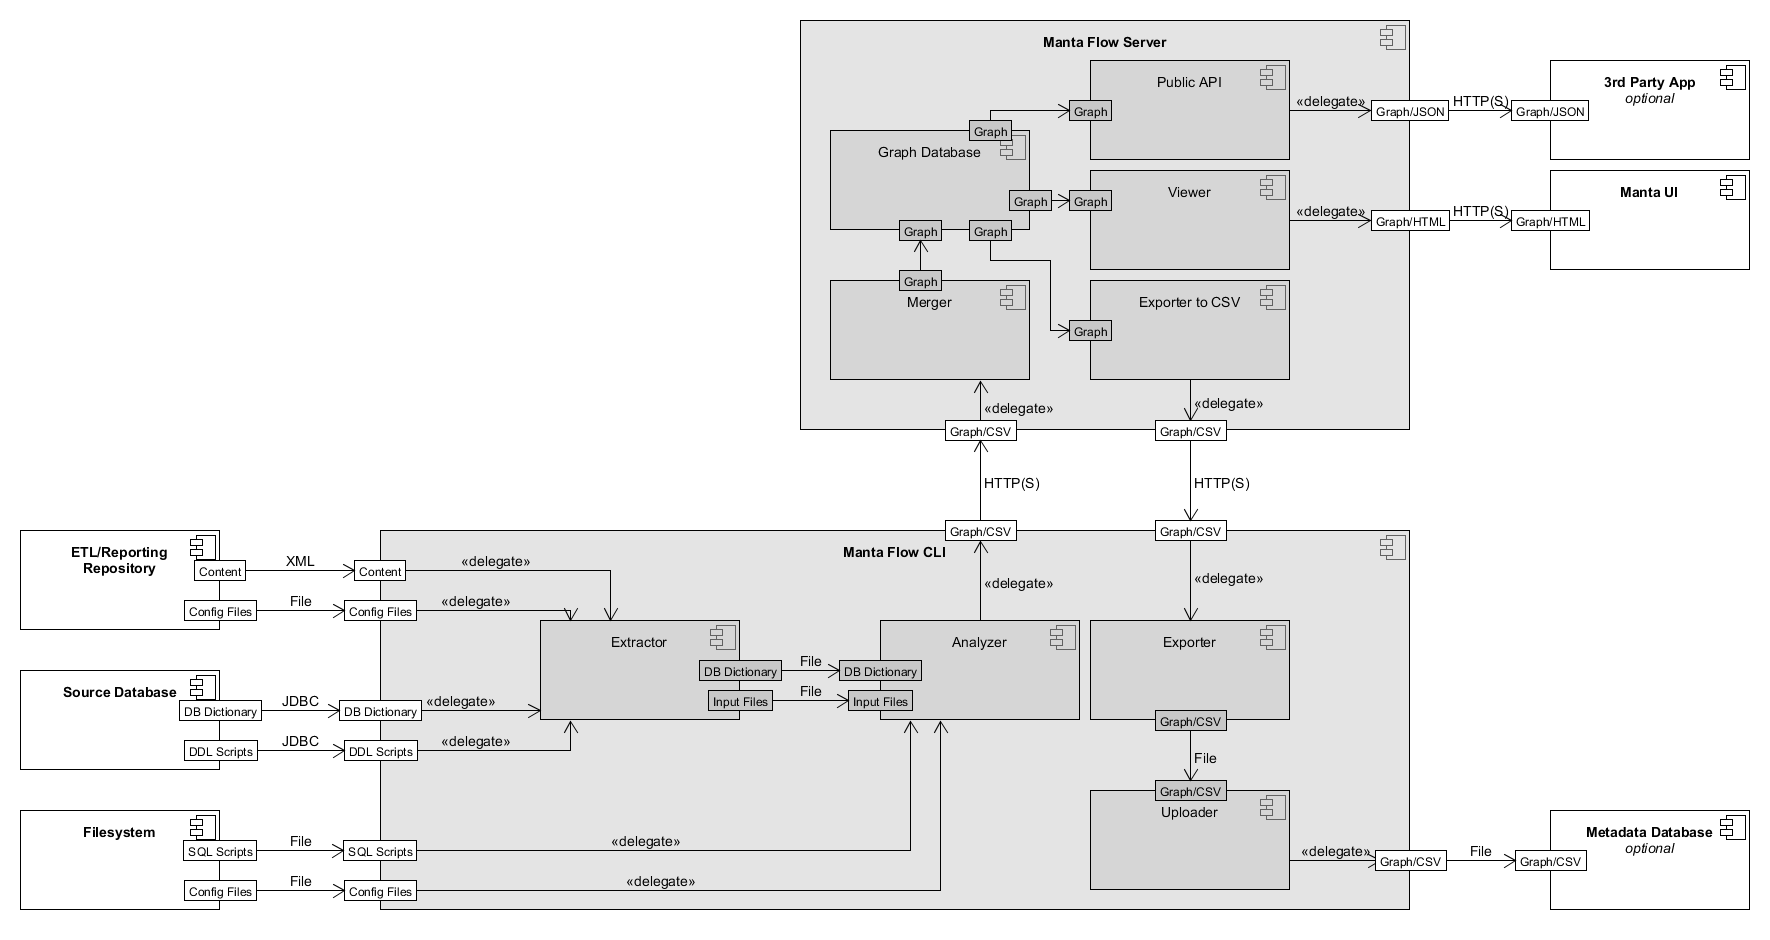
\includegraphics[width=14cm]{figures/flow_comp}
\caption{Architektura \textit{Manta Flow}}
\label{fig:ana-flow-comp}
\end{center}
\end{figure}

\begin{figure}
\begin{center}
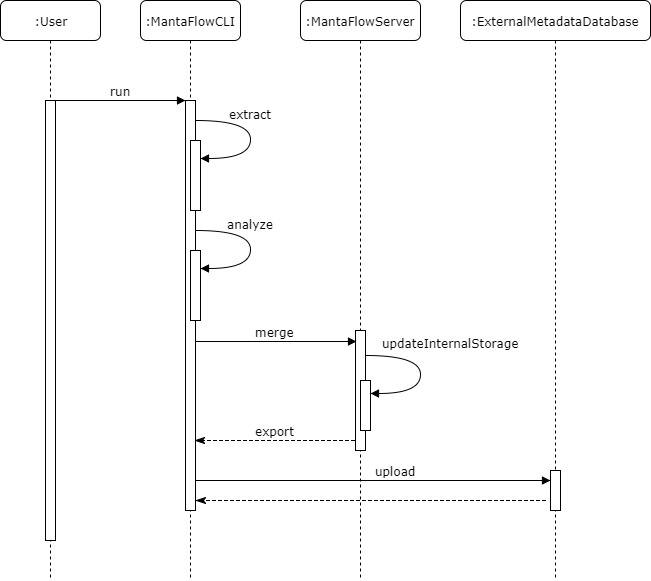
\includegraphics[width=14cm]{figures/flow_seq}
\caption{Interakce mezi \textit{klientskou} a \textit{serverovou} částí \textit{Manta Flow}}
\label{fig:ana-flow-seq}
\end{center}
\end{figure}

\subsection{Metadatové uložiště}
\label{sec:ana_model}
Jak již bylo zmíněno v úvodu práce (kapitola \ref{sec:uvod}) metadatové uložiště produktu \textit{Manta Flow} je aktuálně implementováno grafovou databází \textit{Titan} (ve verzi 0.4) a je snaha o výměnu této databáze %\cite{TODO Kovar}. 
Než přistoupíme k bližšímu popisu jednotlivých komponent aplikace a jejich interakcí s metadatovým uložištěm (kapitola \ref{sec:ana_interactions}, je třeba nejdříve popsat jeho datový model zobrazený na obrázku \ref{fig:ana-model}. 

% TODO popsat reálné entity 
% TODO je to strom?
% TODO zmínit horizontální filtry?

\begin{figure}
\begin{center}
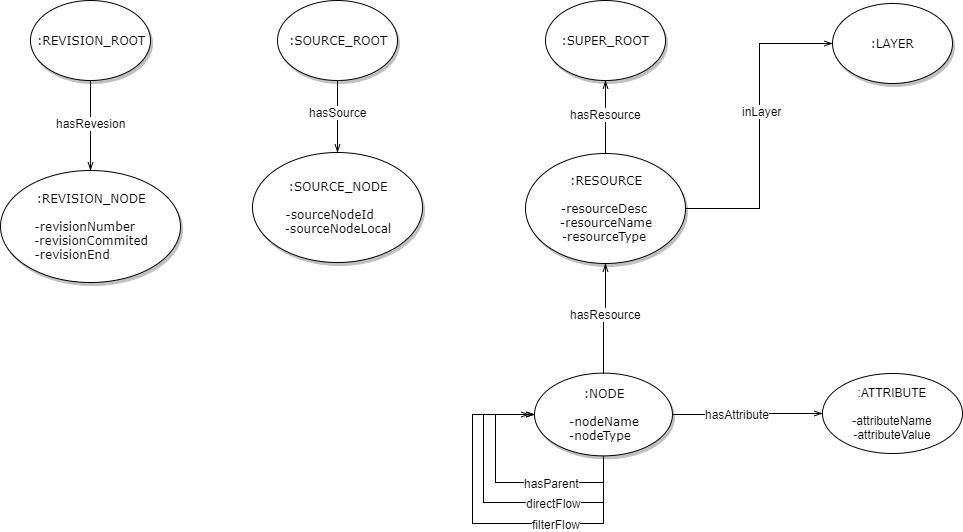
\includegraphics[width=14cm]{figures/model}
\caption{Model grafové databáze}
\label{fig:ana-model}
\end{center}
\end{figure}

Model se skládá z devíti typů uzlů:

\begin{itemize}
	\item{\textit{SUPER\_ROOT}}: Uzel (právě jeden v databázi), který slouží jako umělý kořen všech uzlů typu \textit{RESOURCE}. 
	\item{\textit{RESOURCE}}: Uzly tohoto typu reprezentují zdrojové systémy - zdroje definic objektů, zdrojových kódů, ETL řešení a další.  
	\item{\textit{NODE}}: Uzly typu \textit{NODE} představují reálné objekty zdrojového systému - databáze, tabulky, sloupce, procedury, skripty a další. 
	\item{\textit{LAYER}}: Uzly typu \textit{LAYER} reprezentují vrstvy modelu metadat. Datové toky nalezené při analýze zdrojových kódů jsou vždy ukládány do \textit{fyzické vrstvy}, ze které je potom možné generovat abstraktnější vrstvy modelu datových toků.  
	\item{\textit{ATTRIBUTE}}: Uzly typu \textit{ATTRIBUTE} reprezentují atributy uzlů typu \textit{NODE} - parametry sloupců, popisy databázových objektů a další.
	\item{\textit{SOURCE\_ROOT}}: Uzel (právě jeden v databázi), který slouží jako umělý kořen všech uzlů typu \textit{SOURCE\_NODE}. 
	\item{\textit{SOURCE\_NODE}}: Uzly typu \textit{SOURCE\_NODE} reprezentují soubory se zdrojovými kódy extrahovanými ze zdrojových systémů. 
	\item{\textit{REVISION\_ROOT}}: Uzel (právě jeden v databázi), který slouží jako umělý kořen všech uzlů typu \textit{REVISION\_NODE}. 
	\item{\textit{REVISION\_NODE}}: Uzly typu \textit{ATTRIBUTE} reprezentují revize modelu metadat, definují tedy jeho verzování. Kromě dalších parametrů mají všechny hrany grafu parametry \textit{tranEnd} a \textit{tranStart} definující platnost hran (viz obrázek \ref{fig:ana-model-rev}). Při každé analýze zdrojových systémů (která je prováděna dávkově klientskou částí aplikace) je vytvořena nová revize metadatového uložiště obsahující všechny objekty zdrojových systémů.\footnote{Je snaha tento princip upravit tak, aby byly objekty v metadatovém uložišti minimálně repklikovány \cite{Sykora17}.}  
\end{itemize}

 a osmi typů hran:

 \begin{itemize}
	\item{\textit{hasResource}}: Hrana přiřazuje objekty (uzly typu \textit{NODE}) ke svým zdrojovým systémům (uzlům typu \textit{RESOURCE}). Hrana je také použite k propojení uzlů typu \textit{RESOURCE} s uzlem \textit{RESOURCE\_ROOT}.
	\item{\textit{hasParent}}: Hrana mezi dvěmi uzly typu \textit{NODE} vytvářející klasickou hiearchickou strukturu mezi těmito uzly - strom závislostí objektů zdrojových systémů. 
	\item{\textit{directFlow}}: Hrana mezi dvěmi uzly typu \textit{NODE} říkající, že mezi těmito uzly existuje přímý datový tok (ve směru hrany).
	\item{\textit{filterFlow}}: Hrana mezi dvěmi uzly typu \textit{NODE} říkající, že mezi těmito uzly existuje nepřímý datový tok (ve směru hrany).
	\item{\textit{hasAttribute}}: Hrana přiřazující uzlům typu \textit{NODE} jejich atributy (uzly typu \textit{ATTRIBUTE}).
	\item{\textit{inLayer}}: Hrana typu \textit{inLayer} spojeju zdroje (uzly typu \textit{RESOURCE}) a vrstvy a říká, že zdroj patří do dané vrstvy modelu metadat. 
	\item{\textit{hasSource}}: Hrana je použita k propojení uzlů reprezentujících zdrojové kódy (uzly typu \textit{SOURCE\_NODE}) s uzlem \textit{SOURCE\_ROOT}.
	\item{\textit{hasRevision}}: Hrana je použita k propojení uzlů reprezentujících revize modelu metadat (uzly typu \textit{REVISION\_NODE}) s uzlem \textit{REVISION\_ROOT}.
\end{itemize}

\begin{figure}
\begin{center}
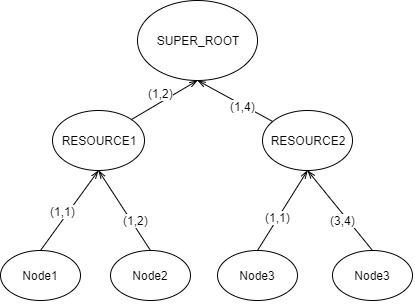
\includegraphics[width=6cm]{figures/model_revisions}
\caption{Způsob verzování modelu metadat}
\label{fig:ana-model-rev}
\end{center}
\end{figure}

% TODO indexy

\subsection{Interakce s metadatovým uložištěm}
\label{sec:ana_interactions}

%TODO cíle podkapitoly
% Cílem je popsat AS-IS stav. 
% Cílem není detailní technický popis všech dotazů do metadatového uložiště, ale spíše obecný popis použitých způsobů manipulace s metadatovým uložištěm a specifických situací. 
% TODO kouknout k Milanovi na ty specifické situace :) 

\subsubsection{Connector}
\label{sec:ana_connector}
Modul, který je nejblíže metadatovému uložišti, tzv. \textbf{connector} má dvě hlavní zodpovědnosti - zajištění připojení k uložišti a provádění dotazů nad ním. 

%Operations
Modul obsahuje sadu základních dotazů, tzv. \textit{operatinos}, mezi které patří například: 
\begin{itemize}
	\item{získání předka uzlu}
	\item{získání atributů uzlu}
	\item{získání sousedních uzlů a hran}
	\item{získání cesty ke kořeni}
	\item{získání podstromu}
\end{itemize} 
Tyto operace přímo přistupují do databáze a pomocí programovacího jazyka \textit{Gremlin}\footnote{Používá se \textit{TinkerPop} ve verzi \textit{2.6.x}.} a jsou na nich postaveny složitější operace nad grafouvou databází. U základních operací nejsou transakce řízeny explicitně, ale implicitně grafovou databází.

% Algorithm
Další částí modulu \textit{connector} jsou tzv. algoritmy, tedy komponenta, pomocí které jsou v metadatovém uložišti hledány samotné datové toky. Tato komponenta řetězí několik grafových algoritmů, přičemž první z nich získá z metadatového uložiště podmnožinu datových toků, která je dalšími algoritmy filtrována a omezována. Tímto způsobem vzniká tzv. \textit{referenční view} - objekt obsahující kompletní graf datových toků pro zadané výchozí uzly a směr datových toků. To je pak využíváno dalšími moduly aplikace, například \textit{viewerem} (viz \ref{sec:ana_viewer}), který dle parametrů zadaných ve webové aplikaci graf datových toků vizualizuje.   
Jednotlivé algoritmy používají výše popsané základní operace a v některých případech také sami dotazují metadatové uložiště přímo pomocí jazyka \textit{Gremlin}. 

% Traversal
Posledním způsobem manipulace s metadatovým uložištěm, který modul umožňuje je přístup pomocí \textit{traverserů}. Ty pracují na obecném principu \textit{traversování} grafů popsaném v kapitole \ref{sec:gdb-dotazy}. V tomto případě ale celý průchod grafem není realizován samotnou grafovou databází, ale \textit{Java} kódem, přičemž grafová databáze je dotazována pouze na dílčí informace - například na okolní uzly. \textit{Traversery} jsou používány v případech, kdy je manipulováno s větší částí grafové databáze, například při jejím exportu. Tyto operace jsou realizovány \textit{vizitory} - každý uzel, který je procházen \textit{traverserem} je následně obsloužen \textit{vizitorem}, který provede požadovanou operaci (jedná se o návrhový vzor \textit{Visitor} - viz \cite{Gamma94}). Obě tyto části, tedy procházení grafu \textit{traverserem} i obsloužení všech objektů \textit{visitorem} je prováděno za pomocí základních grafových operací definovaných výše. Zároveň je ale také z tohoto kontextu grafová databáze dotazována přímo pomocí jazyka \textit{Gremlin}. Jedná se ale spíše o jednoduché dotazy na dohledání uzlů, jejich atributů apod. 

\subsubsection{Merger}
\textit{Merger} je modul, který je používán při analýze zdrojových systémů. Slouží k zanesení výsledků dílčích analýz jednotlivých částí (např. skriptů) zdrojových systémů do metadatového uložiště. 

% TODO
%  Vstupy - co vše obsahuje jeden mergovaný graf? 
% Vstup - serializovaný graf - byte[]
%  - co je scriptmetadata? 

Vlastní operace \textit{merge}\footnote{Operace \textit{merge} má v kontextu aplikace \textit{Manta Flow} obdobný význam, jako například v \textit{SQL}: pokud objekt není uložen v persistentní vrstvě, je do ní uložen (\textit{insert}), jinak je aktualizován (\textit{update}).} lze zjednodušeně popsat pseudokódem \ref{alg_merger}. Ten je uveden především kvůli složitému mode zanořování transakcí, jehož účelem je vyvážení efektivity operace \textit{merge} a zároveň umožňení provádění dotazů do metadatového uložiště jinými částmi aplikace. % TODO blíže popsat použitý transakční model

Operace se také chová různě v případě, kdy je umožňěno verzovaní metadatového uložiště (a to tak obsahuje více revízí) a kdy je vypnuto. V případě zapnutého verzování je \textit{merge} prováděn vždy do nové revize, pokud je verzování vypnuté, je prováděn do hlavní (jediné) revize. 

Samotné \textit{merge} operace nad objekty (uzly, hranami, atributy, ...) jsou prováděny přímo do grafové databáze pomocí jazyka \textit{Gremlin}. K přístupu do metadadtového uložiště se tedy nevyužívá modul k tomu předurčený - \textit{Connector} (viz \ref{sec:ana_connector}).

\begin{algorithm} 
\caption{Merger pseudocode}
\label{alg_merger}
\begin{algorithmic}
	\State $beginWriteTransaction()$
	\State $revision\gets getNewestRevision()$
	\If {$revision.isOpen()$}
		\State $beginWriteTransaction()$
		\ForAll{$script in scripts$} 
			\State $beginWriteTransaction()$
			\State $merge(script)$	
			\State $conditionalCommit()$
		\EndFor
		\State $beginWriteTransaction()$
		\ForAll{$object in objects$} 
			\State $beginWriteTransaction()$
			\State $merge(object)$	
			\State $occasionalCommit()$
		\EndFor
		\State $commit()$	
	\EndIf
	\State $commit()$
\end{algorithmic}
\end{algorithm}


\subsubsection{Query}
% TODO 
% Dotazy 
% - proč se flow hledá pro interval revízí a ne jen jednu revizi?
Modulem zajišťujícím dotazy do metadatového uložiště je \textbf{Query}. Ten umožňuje několik jednoduchých dotazů do metadatového uložiště a komplexní dotaz pro nalezení datových toků, který blíže popíšeme.  


\subsubsection{Viewer}
\label{sec:ana_viewer}
\textit{Viewer} je modul sloužící k poskytování dat uživatelskému rozhraní aplikace (klientské části webové aplikace). Jeho nejčastější interakce s metadatovým uložištěm je dotaz na \textit{referenční view} dle parametrů zadaných uživatelem. To je prováděno pomocí algoritmů definovaných v modulu \textit{connector} (viz \ref{sec:ana_connector}) a modulu \textit{query}, který obsahuje pomocné funkce pro hledání datových toků (resp. \textit{referenčního view}) a také konfiguraci algoritmů poskytovaných \textit{connectorem}.  , také částečně přímo interaguje s metadatovým uložištěm. 

Kromě toho \textit{viewer} dotazuje metadatové uložiště o další informace, které následně propaguje do uživatelského rozhraní - především o informace o revizích metadatového uložiště a o objekty zdrojových systémů, pomocí kterých uživatel vybírá výchozí uzly pro hledání datových toků (\textit{referenčního view}). Informace o revizích metadatového uložiště jsou dohledávány pomocí základních operací definovaných v modulu \textit{connector} (viz \ref{sec:ana_connector}) a pomocí přímých dotazů do metadatového uložiště pomocí jazyka \textit{Gremlin} s explicitního řízení transakcí. Pro vyhledávání objektů zdrojových systémů (v metadatovém uložišti uzly typu \textit{NODE}, viz \ref{sec:ana_model}) je použito vyhledávání pomocí fulltextového indexu implementovaného pomocí \textit{Apache Lucene}\footnote{\url{https://lucene.apache.org/}}. Ten indexuje uzly v metadatovém uložišti podle jejich názvu a umožňuje jejich rychlé vyhledávání. 


\subsubsection{Public API}
% TODO
% Public API 




\subsubsection{Exporter}
% TODO 
% Export to CSV (exporter)

% TODO
% dump


% TODO POPIS API jednotlivých databází
\subsection{GDB API} %TODO CHANGE

%TODO
\subsection{Požadavky}
%security 
% - podle rolí
% - nevidím flow v cizích systémech, ale vidím, že z vlastního tam flow vede

% - Není nutné upravovat algoritmus pro hledání flow  				--- stačí najít kompletní flow se všmi objekty a odfiltrovat zakázané.
% - Úprava algoritmu pro hledání flow by alg. nezrychlila 			--- stejně by bylo nutné hledat přes zakázané objekty (pro případ, že za nimi jsou ještě viditelné objekty, které jsou součástí flow)
% ==> Neupravovat algoritmy, natož DB dotazy
% ==> Nalezená flow by měla být filtrována -> sw. vrstva - na jaké úrovni? 
% - Filtrovat by se mělo až ve chvíli, kdy je flow kompletní 
% - - 


